% This LaTeX document needs to be compiled with XeLaTeX.
\documentclass[10pt]{article}
\usepackage[utf8]{inputenc}
\usepackage{graphicx}
\usepackage[export]{adjustbox}
\graphicspath{ {./images/} }
\usepackage{amsmath}
\usepackage{amsfonts}
\usepackage{amssymb}
\usepackage[version=4]{mhchem}
\usepackage{stmaryrd}
\usepackage{multirow}
\usepackage[fallback]{xeCJK}
\usepackage{polyglossia}
\usepackage{fontspec}
\setCJKmainfont{Noto Serif CJK JP}

\setmainlanguage{polish}
\setmainfont{CMU Serif}

\title{WYPEとNIA ZDAJĄCY }

\author{}
\date{}


\newcommand\Varangle{\mathop{{<\!\!\!\!\!\text{\small)}}\:}\nolimits}

\begin{document}
\maketitle
\section*{KOD}
PESEL\\
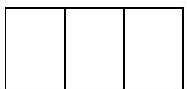
\includegraphics[max width=\textwidth, center]{2024_11_21_46d945490f1b2eff1c8eg-01(1)}

\begin{center}
\begin{tabular}{|l|l|l|l|l|l|l|l|l|l|l|}
\hline
 &  &  &  &  &  &  &  &  &  &  \\
\hline
\end{tabular}
\end{center}

\section*{Miejsce na naklejkę.}
Sprawdż, czy kod na naklejce to E-100.\\
Jeżeli tak - przyklej naklejkę. Jeżeli nie - zgłoś to nauczycielowi.

\section*{EGZAMIN MATURALNY Z MATEMATYKI POZIOM PODSTAWOWY}
DATA: 5 maja 2021 r. GODZINA ROZPOCZECIA: 9:00\\
CZAS PRACY: 170 minut\\
LICZBA PUNKTÓW DO UZYSKANIA: 45

\section*{WYPEŁNIA ZESPÓŁ NADZORUJACY}
Uprawnienia zdającego do:\\
dostosowania zasad oceniania dostosowania w zw. z dyskalkulią nieprzenoszenia zaznaczeń na kartę.\\
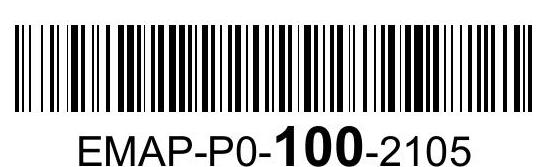
\includegraphics[max width=\textwidth, center]{2024_11_21_46d945490f1b2eff1c8eg-01}

\section*{Instrukcja dla zdającego}
\begin{enumerate}
  \item Sprawdź, czy arkusz egzaminacyjny zawiera 25 stron (zadania 1-35). Ewentualny brak zgłoś przewodniczącemu zespołu nadzorującego egzamin.
  \item Na tej stronie oraz na karcie odpowiedzi wpisz swój numer PESEL i przyklej naklejkę z kodem.
  \item Nie wpisuj żadnych znaków w części przeznaczonej dla egzaminatora.
  \item Rozwiązania zadań i odpowiedzi wpisuj w miejscu na to przeznaczonym.
  \item Odpowiedzi do zadań zamkniętych (1-28) zaznacz na karcie odpowiedzi w części karty przeznaczonej dla zdającego. Zamaluj \(\square\) pola do tego przeznaczone. Błędne zaznaczenie otocz kółkiem ( i zaznacz właściwe.
  \item Pamiętaj, że pominięcie argumentacji lub istotnych obliczeń w rozwiązaniu zadania otwartego (29-35) może spowodować, że za to rozwiązanie nie otrzymasz pełnej liczby punktów.
  \item Pisz czytelnie i używaj tylko długopisu lub pióra z czarnym tuszem lub atramentem.
  \item Nie używaj korektora, a błędne zapisy wyraźnie przekreśl.
  \item Pamiętaj, że zapisy w brudnopisie nie będą oceniane.
  \item Możesz korzystać z zestawu wzorów matematycznych, cyrkla i linijki oraz kalkulatora prostego.
\end{enumerate}

W każdym z zadań od 1. do 28. wybierz i zaznacz na karcie odpowiedzi poprawną odpowiedź.

\section*{Zadanie 1. (0-1)}
Liczba \(100^{5} \cdot(0,1)^{-6}\) jest równa\\
A. \(10^{13}\)\\
B. \(10^{16}\)\\
C. \(10^{-1}\)\\
D. \(10^{-30}\)

\section*{Zadanie 2. (0-1)}
Liczba 78 stanowi 150\% liczby \(c\). Wtedy liczba \(c\) jest równa\\
A. 60\\
B. 52\\
C. 48\\
D. 39

\section*{Zadanie 3. (0-1)}
Rozważamy przedziały liczbowe \((-\infty, 5)\) i \(\langle-1,+\infty)\). lle jest wszystkich liczb całkowitych, które należą jednocześnie do obu rozważanych przedziałów?\\
A. 6\\
B. 5\\
C. 4\\
D. 7

\section*{Zadanie 4. (0-1)}
Suma \(2 \log \sqrt{10}+\log 10^{3}\) jest równa\\
A. 2\\
B. 3\\
C. 4\\
D. 5

\section*{Zadanie 5. (0-1)}
Różnica 0,(3) \(-\frac{23}{33}\) jest równa\\
A. \(-0,(39)\)\\
B. \(-\frac{39}{100}\)\\
C. \(-0,36\)\\
D. \(-\frac{4}{11}\)

\section*{Zadanie 6. (0-1)}
Zbiorem wszystkich rozwiązań nierówności \(\frac{2-x}{2}-2 x \geq 1\) jest przedział\\
A. \(\langle 0,+\infty)\)\\
B. \((-\infty, 0)\)\\
C. \((-\infty, 5)\)\\
D. \(\left(-\infty, \frac{1}{3}\right)\)

\section*{BRUDNOPIS (nie podlega ocenie)}
\begin{center}

\includegraphics[max width=\textwidth]{2024_11_21_46d945490f1b2eff1c8eg-03}
\end{center}

\section*{Zadanie 7. (0-1)}
Na poniższym rysunku przedstawiono wykres funkcji \(f\) określonej w zbiorze \(\langle-6,5\rangle\).\\
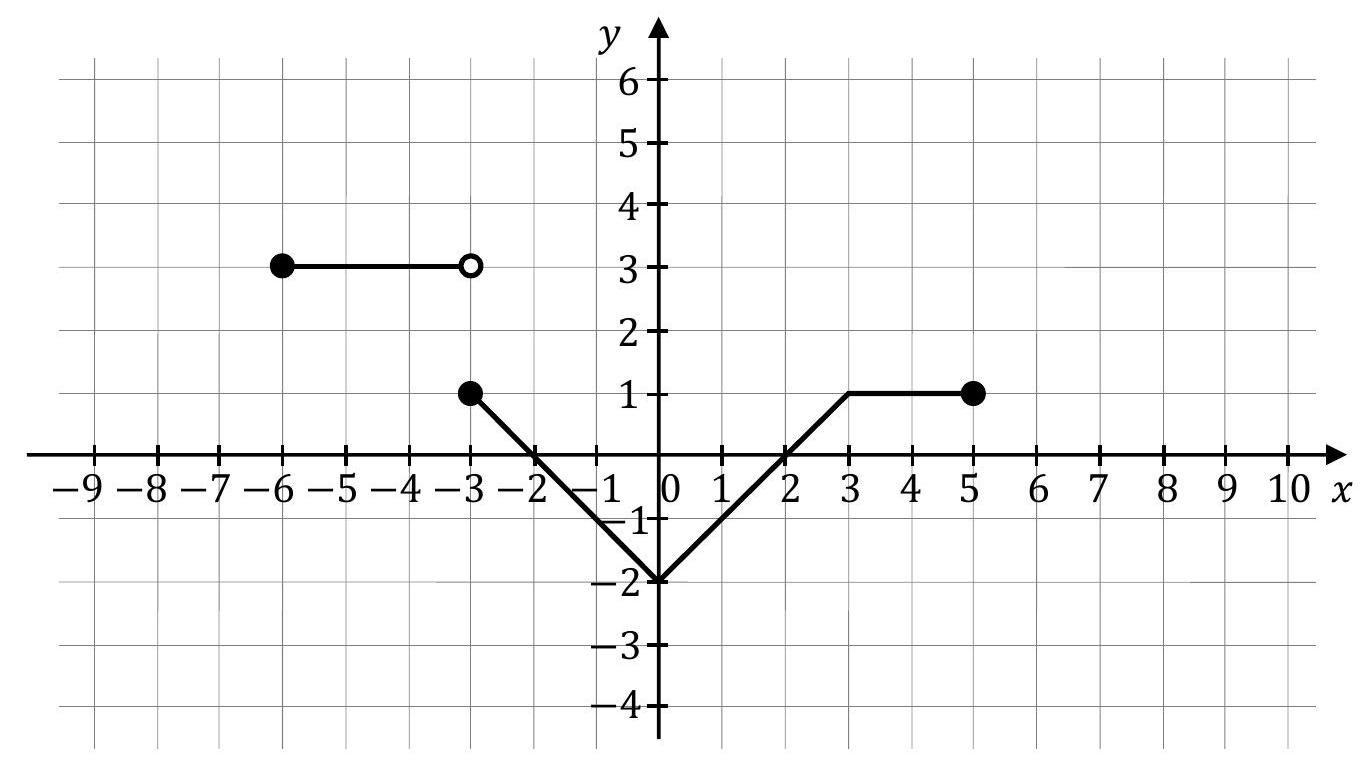
\includegraphics[max width=\textwidth, center]{2024_11_21_46d945490f1b2eff1c8eg-04(1)}

Funkcja \(\quad g\) jest określona wzorem \(g(x)=f(x)-2\) dla \(x \in\langle-6,5\rangle\). Wskaż zdanie prawdziwe.\\
A. Liczba \(f(2)+g(2)\) jest równa \((-2)\).\\
B. Zbiory wartości funkcji \(f\) i \(g\) są równe.\\
C. Funkcje \(f\) i \(g\) mają te same miejsca zerowe.\\
D. Punkt \(P=(0,-2)\) należy do wykresów funkcji \(f\) i \(g\).

\section*{Zadanie 8. (0-1)}
Na rysunku obok przedstawiono geometryczną interpretację jednego z niżej zapisanych układów równań. Wskaż ten układ, którego geometryczną interpretację przedstawiono na rysunku.\\
A. \(\left\{\begin{array}{l}y=x+1 \\ y=-2 x+4\end{array}\right.\)\\
B. \(\left\{\begin{array}{l}y=x-1 \\ y=2 x+4\end{array}\right.\)\\
C. \(\left\{\begin{array}{l}y=x-1 \\ y=-2 x+4\end{array}\right.\)\\
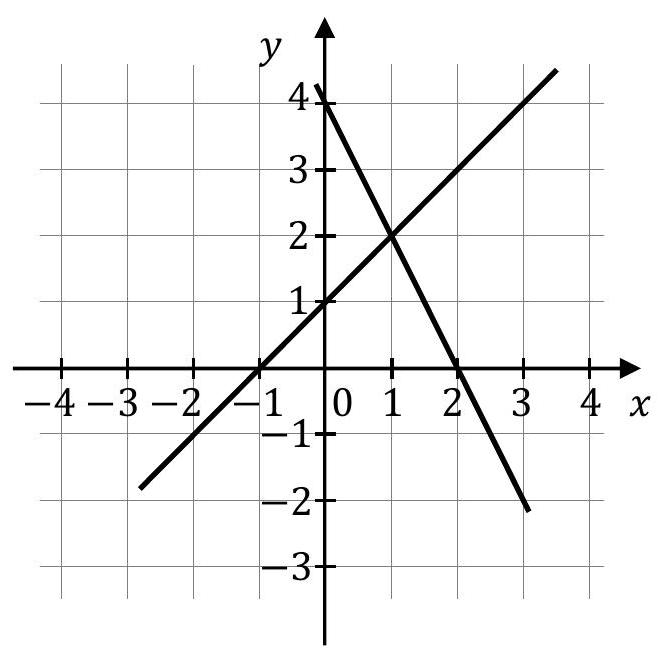
\includegraphics[max width=\textwidth, center]{2024_11_21_46d945490f1b2eff1c8eg-04}\\
D. \(\left\{\begin{array}{l}y=x+1 \\ y=2 x+4\end{array}\right.\)

\section*{BRUDNOPIS (nie podlega ocenie)}
\begin{center}

\includegraphics[max width=\textwidth]{2024_11_21_46d945490f1b2eff1c8eg-05}
\end{center}

\section*{Zadanie 9. (0-1)}
Proste o równaniach \(y=3 x-5\) oraz \(y=\frac{m-3}{2} x+\frac{9}{2}\) są równoległe, gdy\\
A. \(m=1\)\\
B. \(m=3\)\\
C. \(m=6\)\\
D. \(m=9\)

\section*{Zadanie 10. (0-1)}
Funkcja \(f\) jest określona wzorem \(f(x)=\frac{x^{2}}{2 x-2}\) dla każdej liczby rzeczywistej \(x \neq 1\). Wtedy dla argumentu \(x=\sqrt{3}-1\) wartość funkcji \(f\) jest równa\\
A. \(\frac{1}{\sqrt{3}-1}\)\\
B. -1\\
C. 1\\
D. \(\frac{1}{\sqrt{3}-2}\)

\section*{Zadanie 11. (0-1)}
Do wykresu funkcji \(f\) określonej dla każdej liczby rzeczywistej \(x\) wzorem \(f(x)=3^{x}-2\) należy punkt o współrzędnych\\
A. \((-1,-5)\)\\
B. \((0,-2)\)\\
C. \((0,-1)\)\\
D. \((2,4)\)

\section*{Zadanie 12. (0-1)}
Funkcja kwadratowa \(f\) określona wzorem \(f(x)=-2(x+1)(x-3)\) jest malejąca w przedziale\\
A. \((1,+\infty)\)\\
B. \((-\infty, 1)\)\\
C. \((-\infty,-8)\)\\
D. \((-8,+\infty)\)

\section*{Zadanie 13. (0-1)}
Trzywyrazowy ciąg \(\left(15,3 x, \frac{5}{3}\right)\) jest geometryczny i wszystkie jego wyrazy są dodatnie. Stąd wynika, że\\
A. \(x=\frac{3}{5}\)\\
B. \(x=\frac{4}{5}\)\\
C. \(x=1\)\\
D. \(x=\frac{5}{3}\)

\section*{Zadanie 14. (0-1)}
Ciąg ( \(b_{n}\) ) jest określony wzorem \(b_{n}=3 n^{2}-25 n\) dla każdej liczby naturalnej \(n \geq 1\). Liczba niedodatnich wyrazów ciągu ( \(b_{n}\) ) jest równa\\
A. 14\\
B. 13\\
C. 9\\
D. 8

\section*{BRUDNOPIS (nie podlega ocenie)}
\begin{center}

\includegraphics[max width=\textwidth]{2024_11_21_46d945490f1b2eff1c8eg-07}
\end{center}

Zadanie 15. (0-1)\\
Ciąg arytmetyczny \(\left(a_{n}\right)\) jest określony dla każdej liczby naturalnej \(n \geq 1\). Trzeci i piąty wyraz ciągu spełniają warunek \(a_{3}+a_{5}=58\). Wtedy czwarty wyraz tego ciągu jest równy\\
A. 28\\
B. 29\\
C. 33\\
D. 40

\section*{Zadanie 16. (0-1)}
Dla każdego kąta ostrego \(\alpha\) iloczyn \(\frac{\cos \alpha}{1-\sin ^{2} \alpha} \cdot \frac{1-\cos ^{2} \alpha}{\sin \alpha}\) jest równy\\
A. \(\sin \alpha\)\\
B. \(\operatorname{tg} \alpha\)\\
C. \(\cos \alpha\)\\
D. \(\sin ^{2} \alpha\)

\section*{Zadanie 17. (0-1)}
Prosta \(k\) jest styczna w punkcie \(A\) do okręgu o środku \(O\). Punkt \(B\) leży na tym okręgu i miara kąta \(A O B\) jest równa \(80^{\circ}\). Przez punkty \(O\) i \(B\) poprowadzono prostą, która przecina prostą \(k\) w punkcie \(C\) (zobacz rysunek).\\
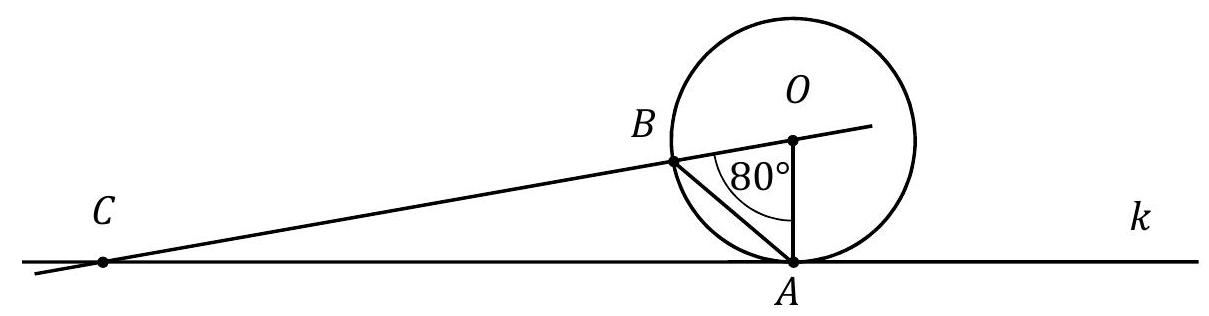
\includegraphics[max width=\textwidth, center]{2024_11_21_46d945490f1b2eff1c8eg-08(1)}

Miara kąta \(B A C\) jest równa\\
A. \(10^{\circ}\)\\
B. \(30^{\circ}\)\\
C. \(40^{\circ}\)\\
D. \(50^{\circ}\)

\section*{Zadanie 18. (0-1)}
Przyprostokątna \(A C\) trójkąta prostokątnego \(A B C\) ma długość 8 oraz \(\operatorname{tg} \alpha=\frac{2}{5}\) (zobacz rysunek).\\
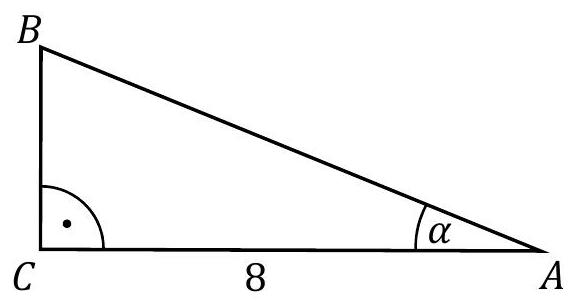
\includegraphics[max width=\textwidth, center]{2024_11_21_46d945490f1b2eff1c8eg-08}

Pole tego trójkąta jest równe\\
A. 12\\
B. \(\frac{37}{3}\)\\
C. \(\frac{62}{5}\)\\
D. \(\frac{64}{5}\)

\section*{BRUDNOPIS (nie podlega ocenie)}
\begin{center}

\includegraphics[max width=\textwidth]{2024_11_21_46d945490f1b2eff1c8eg-09}
\end{center}

Zadanie 19. (0-1)\\
Pole pewnego trójkąta równobocznego jest równe \(\frac{4 \sqrt{3}}{9}\). Obwód tego trójkąta jest równy\\
A. 4\\
B. 2\\
C. \(\frac{4}{3}\)\\
D. \(\frac{2}{3}\)

\section*{Zadanie 20. (0-1)}
W trójkącie \(A B C\) bok \(B C\) ma długość 13, a wysokość \(C D\) tego trójkąta dzieli bok \(A B\) na odcinki o długościach \(|A D|=3\) i \(|B D|=12\) (zobacz rysunek obok). Długość boku \(A C\) jest równa\\
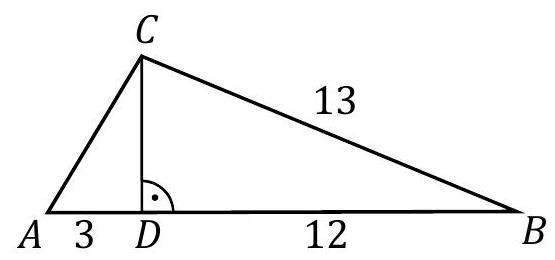
\includegraphics[max width=\textwidth, center]{2024_11_21_46d945490f1b2eff1c8eg-10}\\
A. \(\sqrt{34}\)\\
B. \(\frac{13}{4}\)\\
C. \(2 \sqrt{14}\)\\
D. \(3 \sqrt{45}\)

\section*{Zadanie 21. (0-1)}
Punkty \(A, B, C\) i \(D\) leżą na okręgu o środku \(S\). Miary kątów \(S B C, B C D, C D A\) są równe odpowiednio: \(|\Varangle S B C|=60^{\circ},|\Varangle B C D|=110^{\circ},|\Varangle C D A|=90^{\circ}\) (zobacz rysunek).\\
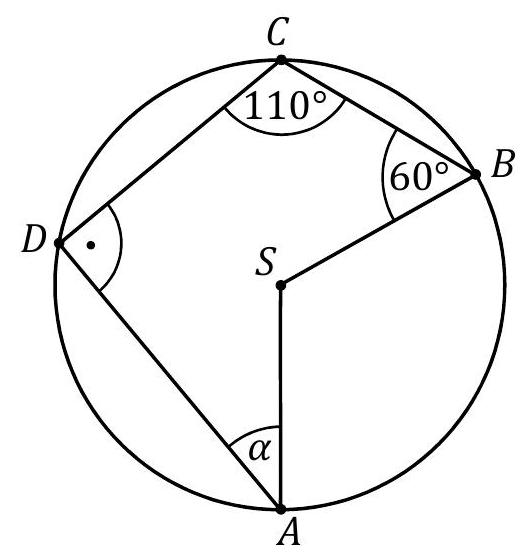
\includegraphics[max width=\textwidth, center]{2024_11_21_46d945490f1b2eff1c8eg-10(1)}

Wynika stąd, że miara \(\alpha\) kąta \(D A S\) jest równa\\
A. \(25^{\circ}\)\\
B. \(30^{\circ}\)\\
C. \(35^{\circ}\)\\
D. \(40^{\circ}\)

\section*{BRUDNOPIS (nie podlega ocenie)}
\begin{center}

\includegraphics[max width=\textwidth]{2024_11_21_46d945490f1b2eff1c8eg-11}
\end{center}

Zadanie 22. (0-1)\\
W równoległoboku \(A B C D\), przedstawionym na rysunku, kąt \(\alpha\) ma miarę \(70^{\circ}\).\\
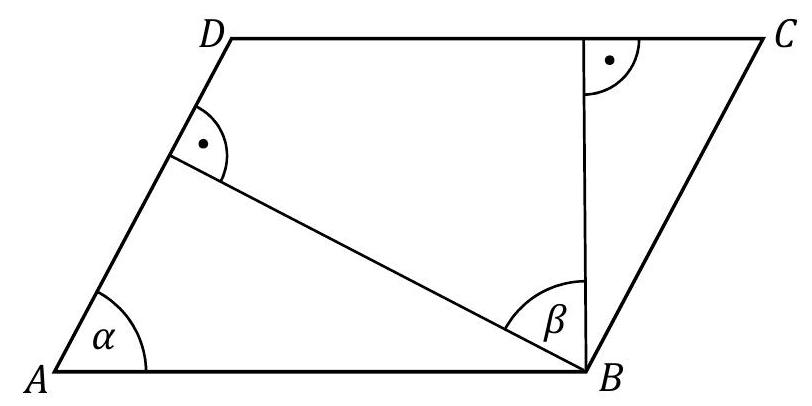
\includegraphics[max width=\textwidth, center]{2024_11_21_46d945490f1b2eff1c8eg-12(2)}

Wtedy kąt \(\beta\) ma miarę\\
A. \(80^{\circ}\)\\
B. \(70^{\circ}\)\\
C. \(60^{\circ}\)\\
D. \(50^{\circ}\)

\section*{Zadanie 23. (0-1)}
W każdym \(n\)-kącie wypukłym \((n \geq 3)\) liczba przekątnych jest równa \(\frac{n(n-3)}{2}\). Wielokątem wypukłym, w którym liczba przekątnych jest o 25 większa od liczby boków, jest\\
A. siedmiokąt.\\
B. dziesięciokąt.\\
C. dwunastokąt.\\
D. piętnastokąt.

\section*{Zadanie 24. (0-1)}
Pole figury \(F_{1}\) złożonej \(z\) dwóch stycznych zewnętrznie kół o promieniach 1 i 3 jest równe polu figury \(F_{2}\) złożonej z dwóch stycznych zewnętrznie kół o promieniach długości \(r\) (zobacz rysunek).

Figura \(F_{1}\)\\
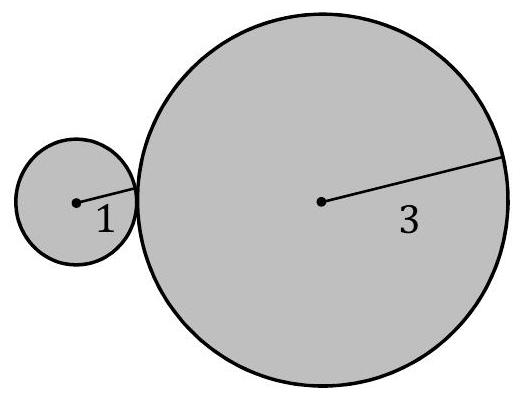
\includegraphics[max width=\textwidth, center]{2024_11_21_46d945490f1b2eff1c8eg-12}

Figura \(F_{2}\)\\
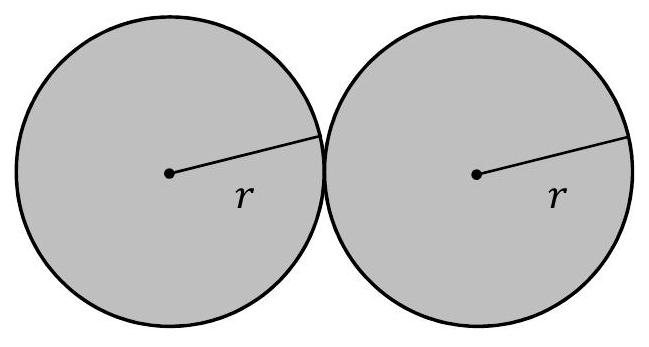
\includegraphics[max width=\textwidth, center]{2024_11_21_46d945490f1b2eff1c8eg-12(1)}

Długość \(r\) promienia jest równa\\
A. \(\sqrt{3}\)\\
B. 2\\
C. \(\sqrt{5}\)\\
D. 3

\section*{BRUDNOPIS (nie podlega ocenie)}
\begin{center}

\includegraphics[max width=\textwidth]{2024_11_21_46d945490f1b2eff1c8eg-13}
\end{center}

\section*{Zadanie 25. (0-1)}
Punkt \(A=(3,-5)\) jest wierzchołkiem kwadratu \(A B C D\), a punkt \(M=(1,3)\) jest punktem przecięcia się przekątnych tego kwadratu. Wynika stąd, że pole kwadratu \(A B C D\) jest równe\\
A. 68\\
B. 136\\
C. \(2 \sqrt{34}\)\\
D. \(8 \sqrt{34}\)

\section*{Zadanie 26. (0-1)}
Z wierzchołków sześcianu ABCDEFGH losujemy jednocześnie dwa różne wierzchołki. Prawdopodobieństwo tego, że wierzchołki te będą końcami przekątnej sześcianu ABCDEFGH, jest równe\\
A. \(\frac{1}{7}\)\\
B. \(\frac{4}{7}\)\\
C. \(\frac{1}{14}\)\\
D. \(\frac{3}{7}\)

\section*{Zadanie 27. (0-1)}
Wszystkich liczb naturalnych trzycyfrowych, większych od 700, w których każda cyfra należy do zbioru \(\{1,2,3,7,8,9\}\) i żadna cyfra się nie powtarza, jest\\
A. 108\\
B. 60\\
C. 40\\
D. 299

\section*{Zadanie 28. (0-1)}
Sześciowyrazowy ciąg liczbowy (1, \(2,2 x, x+2,5,6)\) jest niemalejący. Mediana wyrazów tego ciągu jest równa 4. Wynika stąd, że\\
A. \(x=1\)\\
B. \(x=\frac{3}{2}\)\\
C. \(x=2\)\\
D. \(x=\frac{8}{3}\)

\section*{BRUDNOPIS (nie podlega ocenie)}
\begin{center}

\includegraphics[max width=\textwidth]{2024_11_21_46d945490f1b2eff1c8eg-15}
\end{center}

Zadanie 29. (0-2)\\
Rozwiąż nierówność:

\[
x^{2}-5 x \leq 14
\]

\begin{center}

\includegraphics[max width=\textwidth]{2024_11_21_46d945490f1b2eff1c8eg-16}
\end{center}

Odpowiedź:

Zadanie 30. (0-2)\\
Wykaż, że dla każdych trzech dodatnich liczb \(a, b\) i \(c\) takich, że \(a<b\), spełniona jest nierówność

\[
\frac{a}{b}<\frac{a+c}{b+c}
\]

\begin{center}

\includegraphics[max width=\textwidth]{2024_11_21_46d945490f1b2eff1c8eg-17}
\end{center}

\begin{center}
\begin{tabular}{|c|c|c|c|}
\hline
\multirow{2}{*}{\begin{tabular}{c}
Wypełnia \\
egzaminator \\
\end{tabular}} & Nr zadania & 29. & 30. \\
\cline { 2 - 4 }
 & Maks. liczba pkt & 2 & 2 \\
\cline { 2 - 4 }
 & Uzyskana liczba pkt &  &  \\
\hline
\end{tabular}
\end{center}

Zadanie 31. (0-2)\\
Funkcja liniowa \(f\) przyjmuje wartość 2 dla argumentu 0 , a ponadto \(f(4)-f(2)=6\). Wyznacz wzór funkcji \(f\).\\

\includegraphics[max width=\textwidth, center]{2024_11_21_46d945490f1b2eff1c8eg-18}

Odpowiedź: \(\qquad\)

Zadanie 32. (0-2)\\
Rozwiąż równanie:

\[
\frac{3 x+2}{3 x-2}=4-x
\]

\begin{center}
\begin{tabular}{|c|c|c|c|c|c|c|c|c|c|c|c|c|c|c|c|c|c|c|c|c|c|c|c|}
\hline
 &  &  &  &  &  &  &  &  &  &  &  &  &  &  &  &  &  &  &  &  &  &  &  \\
\hline
 &  &  &  &  &  &  &  &  &  &  &  &  &  &  &  &  &  &  &  &  &  &  &  \\
\hline
 &  &  &  &  &  &  &  &  &  &  &  &  &  &  &  &  &  &  &  &  &  &  &  \\
\hline
 &  &  &  &  &  &  &  &  &  &  &  &  &  &  &  &  &  &  &  &  &  &  &  \\
\hline
 &  &  &  &  &  &  &  &  &  &  &  &  &  &  &  &  &  &  &  &  &  &  &  \\
\hline
 &  &  &  &  &  &  &  &  &  &  &  &  &  &  &  &  &  &  &  &  &  &  &  \\
\hline
 &  &  &  &  &  &  &  &  &  &  &  &  &  &  &  &  &  &  &  &  &  &  &  \\
\hline
 &  &  &  &  &  &  &  &  &  &  &  &  &  &  &  &  &  &  &  &  &  &  &  \\
\hline
 &  &  &  &  &  &  &  &  &  &  &  &  &  &  &  &  &  &  &  &  &  &  &  \\
\hline
 &  &  &  &  &  &  &  &  &  &  &  &  &  &  &  &  &  &  &  &  &  &  &  \\
\hline
 &  &  &  &  &  &  &  &  &  &  &  &  &  &  &  &  &  &  &  &  &  &  &  \\
\hline
 &  &  &  &  &  &  &  &  &  &  &  &  &  &  &  &  &  &  &  &  &  &  &  \\
\hline
 &  &  &  &  &  &  &  &  &  &  &  &  &  &  &  &  &  &  &  &  &  &  &  \\
\hline
 &  &  &  &  &  &  &  &  &  &  &  &  &  &  &  &  &  &  &  &  &  &  &  \\
\hline
 &  &  &  &  &  &  &  &  &  &  &  &  &  &  &  &  &  &  &  &  &  &  &  \\
\hline
 &  &  &  &  &  &  &  &  &  &  &  &  &  &  &  &  &  &  &  &  &  &  &  \\
\hline
 &  &  &  &  &  &  &  &  &  &  &  &  &  &  &  &  &  &  &  &  &  &  &  \\
\hline
 &  &  &  &  &  &  &  &  &  &  &  &  &  &  &  &  &  &  &  &  &  &  &  \\
\hline
 &  &  &  &  &  &  &  &  &  &  &  &  &  &  &  &  &  &  &  &  &  &  &  \\
\hline
 &  &  &  &  &  &  &  &  &  &  &  &  &  &  &  &  &  &  &  &  &  &  &  \\
\hline
 &  &  &  &  &  &  &  &  &  &  &  &  &  &  &  &  &  &  &  &  &  &  &  \\
\hline
 &  &  &  &  &  &  &  &  &  &  &  &  &  &  &  &  &  &  &  &  &  &  &  \\
\hline
 &  &  &  &  &  &  &  &  &  &  &  &  &  &  &  &  &  &  &  &  &  &  &  \\
\hline
 &  &  &  &  &  &  &  &  &  &  &  &  &  &  &  &  &  &  &  &  &  &  &  \\
\hline
 &  &  &  &  &  &  &  &  &  &  &  &  &  &  &  &  &  &  &  &  &  &  &  \\
\hline
 &  &  &  &  &  &  &  &  &  &  &  &  &  &  &  &  &  &  &  &  &  &  &  \\
\hline
 &  &  &  &  &  &  &  &  &  &  &  &  &  &  &  &  &  &  &  &  &  &  &  \\
\hline
 &  &  &  &  &  &  &  &  &  &  &  &  &  &  &  &  &  &  &  &  &  &  &  \\
\hline
 &  &  &  &  &  &  &  &  &  &  &  &  &  &  &  &  &  &  &  &  &  &  &  \\
\hline
 &  &  &  &  &  &  &  &  &  &  &  &  &  &  &  &  &  &  &  &  &  &  &  \\
\hline
 &  &  &  &  &  &  &  &  &  &  &  &  &  &  &  &  &  &  &  &  &  &  &  \\
\hline
 &  &  &  &  &  &  &  &  &  &  &  &  &  &  &  &  &  &  &  &  &  &  &  \\
\hline
 &  &  &  &  &  &  &  &  &  &  &  &  &  &  &  &  &  &  &  &  &  &  &  \\
\hline
 &  &  &  &  &  &  &  &  &  &  &  &  &  &  &  &  &  &  &  &  &  &  &  \\
\hline
 &  &  &  &  &  &  &  &  &  &  &  &  &  &  &  &  &  &  &  &  &  &  &  \\
\hline
 &  &  &  &  &  &  &  &  &  &  &  &  &  &  &  &  &  &  &  &  &  &  &  \\
\hline
\end{tabular}
\end{center}

Odpowiedź:

\begin{center}
\begin{tabular}{|c|c|c|c|}
\hline
\multirow{2}{*}{\begin{tabular}{c}
Wypełnia \\
egzaminator \\
\end{tabular}} & Nr zadania & 31. & 32. \\
\cline { 2 - 4 }
 & Maks. liczba pkt & 2 & 2 \\
\cline { 2 - 4 }
 & Uzyskana liczba pkt &  &  \\
\hline
\end{tabular}
\end{center}

Zadanie 33. (0-2)\\
Trójkąt równoboczny \(A B C\) ma pole równe \(9 \sqrt{3}\). Prosta równoległa do boku \(B C\) przecina boki \(A B\) i \(A C\)-odpowiednio - w punktach \(K\) i \(L\). Trójkąty \(A B C\) i \(A K L\) są podobne, a stosunek długości boków tych trójkątów jest równy \(\frac{3}{2}\). Oblicz długość boku trójkąta \(A K L\).\\

\includegraphics[max width=\textwidth, center]{2024_11_21_46d945490f1b2eff1c8eg-20}

Odpowiedż: \(\qquad\)

Zadanie 34. (0-2)\\
Gracz rzuca dwukrotnie symetryczną sześcienną kostką do gry i oblicza sumę liczb wyrzuconych oczek. Oblicz prawdopodobieństwo zdarzenia \(A\) polegającego na tym, że suma liczb wyrzuconych oczek jest równa 4 lub 5, lub 6.\\

\includegraphics[max width=\textwidth, center]{2024_11_21_46d945490f1b2eff1c8eg-21}

Odpowiedź: \(\qquad\)

\begin{center}
\begin{tabular}{|c|c|c|c|}
\hline
\multirow{2}{*}{\begin{tabular}{c}
Wypełnia \\
egzaminator \\
\end{tabular}} & Nr zadania & 33. & 34. \\
\cline { 2 - 4 }
 & Maks. liczba pkt & \(\mathbf{2}\) & \(\mathbf{2}\) \\
\cline { 2 - 4 }
 & Uzyskana liczba pkt &  &  \\
\hline
\end{tabular}
\end{center}

Zadanie 35. (0-5)\\
Punkty \(A=(-20,12)\) i \(B=(7,3)\) są wierzchołkami trójkąta równoramiennego \(A B C\), w którym \(|A C|=|B C|\). Wierzchołek \(C\) leży na osi \(O y \quad\) układu współrzędnych. Oblicz współrzędne wierzchołka \(C\) oraz obwód tego trójkąta.\\

\includegraphics[max width=\textwidth, center]{2024_11_21_46d945490f1b2eff1c8eg-22}\\

\includegraphics[max width=\textwidth, center]{2024_11_21_46d945490f1b2eff1c8eg-23}

Odpowiedź:

\begin{center}
\begin{tabular}{|c|c|c|}
\hline
\multirow{2}{*}{\begin{tabular}{c}
Wypełnia \\
egzaminator \\
\end{tabular}} & Nr zadania & 35. \\
\cline { 2 - 3 }
 & Maks. liczba pkt & 5 \\
\cline { 2 - 3 }
 & Uzyskana liczba pkt &  \\
\hline
\end{tabular}
\end{center}

\section*{BRUDNOPIS (nie podlega ocenie)}

\includegraphics[max width=\textwidth, center]{2024_11_21_46d945490f1b2eff1c8eg-24}\\

\includegraphics[max width=\textwidth, center]{2024_11_21_46d945490f1b2eff1c8eg-25}


\end{document}